\documentclass{article}
\usepackage{bm}
\usepackage{amsmath}
\usepackage{graphicx}
\usepackage{mdwlist}
\usepackage[colorlinks=true]{hyperref}
\usepackage{geometry}
\usepackage{kotex}
\geometry{margin=1in}
\geometry{headheight=2in}
\geometry{top=2in}
\usepackage{palatino}
%\renewcommand{\rmdefault}{palatino}
\usepackage{fancyhdr}
\usepackage{indentfirst}

\newcommand{\red}[1]{{\color{red} #1}}
\newcommand{\blue}[1]{{\color{blue} #1}}
\newcommand{\orange}[1]{{\color{orange} #1}}
\newcommand{\purple}[1]{{\color{purple} #1}}

%\pagestyle{fancy}
\rhead{}
\lhead{}
\chead{%
  {\vbox{%
      \vspace{2mm}
      \large
      Statistics Lab 033.020\hfill
\\
      Seoul National University
      \\[4mm]
      \textbf{Assignment \#4} \\
      \texttt{2016-19516, Sangjun Son}
    }
  }
}

%%%%%%%%%%%%%%%%%%%%%%%
\usepackage{xcolor}
\usepackage{listings}
\definecolor{vgreen}{RGB}{104,180,104}
\definecolor{vblue}{RGB}{49,49,255}
\definecolor{vorange}{RGB}{255,143,102}

\lstdefinestyle{r-style}
{
    language=R,
    basicstyle=\footnotesize\ttfamily,
    keywordstyle=\color{vblue},
    identifierstyle=\color{black},
    commentstyle=\color{vgreen},
    numbers=left,
    numberstyle=\tiny\color{black},
    numbersep=10pt,
    tabsize=8,
    moredelim=*[s][\colorIndex]{[}{]},
    literate=*{:}{:}1
}

\lstdefinestyle{out-style}
{
    language=R,
    basicstyle=\footnotesize\ttfamily,
    numbersep=10pt,
    tabsize=8,
    moredelim=*[s][\colorIndex]{[}{]},
    literate=*{:}{:}1
}

\makeatletter
\newcommand*\@lbracket{[}
\newcommand*\@rbracket{]}
\newcommand*\@colon{:}
\newcommand*\colorIndex{%
    \edef\@temp{\the\lst@token}%
    \ifx\@temp\@lbracket \color{black}%
    \else\ifx\@temp\@rbracket \color{black}%
    \else\ifx\@temp\@colon \color{black}%
    \else \color{vorange}%
    \fi\fi\fi
}
\makeatother

\usepackage{trace}
%%%%%%%%%%%%%%%%%%%%%%%

\usepackage{paralist}

\usepackage{todonotes}
\setlength{\marginparwidth}{2.15cm}

\usepackage{tikz}
\usetikzlibrary{positioning,shapes,backgrounds}

\begin{document}

\pagestyle{fancy}

\section*{Example 1 $\sim$ 4}

(\textbf{Example 1}) 주어진 자료는 Iowa의 도시 Ames의 2006년부터 2010년 사이의 부동산 거래내역 자료이다.
5년 동안 이 지역에서 발생한 총 2930건의 부동산 거래내역이 모두 기록되어 있다. 본 예제
에서는 집의 크기를 나타내는 변수인 \texttt{Gr.Liv.Area}를 모집단으로 사용하도록 한다. 주어진 자료는 전체 부동산에 대한 자료이므로 모집단으로 생각할 수 있다. 거래가
이루어진 전체 부동산의 집의 크기의 평균값 ($\mu$)은 얼마인가? 모분산 ($\sigma^2$)은 얼마인가?
\begin{lstlisting}[style={r-style}]
ames = read.csv("ames.csv", header=T)
pop = ames$Gr.Liv.Area

pop.mean = mean(pop); pop.mean
pop.sigma = sd(pop); pop.sigma^2
\end{lstlisting}
\begin{lstlisting}[style={out-style}]
[1] 1499.69
[1] 255539.2
\end{lstlisting}
\emph{Explanation: 지난 과제 3에서 사용한 ames 데이터셋을 활용하여 Gr.Liv.Area 변수값을 새로운 모집단 벡터 pop으로 저장하였다. 모평균과 모표준편차를 각각 pop.mean과 pop.sigma에 저장한 후 모평균이 1,499이고 분산은 255,539임을 확인하였다. } \\

(\textbf{Example 2}) 모집단에서 크기가 60인 랜덤 표본을 선택하자. 모집단 평균에 대한 점추정값은 얼마인가?
\begin{lstlisting}[style={r-style}]
n = 60
pop.sample = sample(pop, n, replace=F)
mean(pop.sample)
\end{lstlisting}
\begin{lstlisting}[style={out-style}]
[1] 1516.433
\end{lstlisting}
\emph{Explanation: 점추정 (point estimation)은 하나는 모수를 한 개의 값으로 추정이다. 모집단의 점추정값을 랜덤 표본의 평균으로 점추정할 수 있다. 모집단 pop에서 랜덤 표본을 sample() 함수를 통해 추출하였고 모평균을 표본평균 1,516으로 추정할 수 있다.} \\

(\textbf{Example 3}) 예제 2에서 선택된 표본을 이용하여 모평균에 대한 95\% 신뢰구간을 구해보자. 이 때, 모분산은 예제 1에서 구한 값을 사용하도록 한다. 이 신뢰구간은 모평균을 포함하는가?
\begin{lstlisting}[style={r-style}]
alpha = 0.05
hi = mean(pop.sample) + qnorm(1-alpha/2)*(pop.sigma/sqrt(n))
lo = mean(pop.sample) - qnorm(1-alpha/2)*(pop.sigma/sqrt(n))
(lo < pop.mean) && (pop.mean < hi)
\end{lstlisting}
\begin{lstlisting}[style={out-style}]
[1] TRUE
\end{lstlisting}
\emph{Explanation: \textbf{중심극한정리, CLT}에 의해 선택된 표본의 크기 $n = 60$ 이 충분히 크므로, 랜덤 표본의 표본평균은 근사적으로 정규분포를 따른다고 할 수 있다. 모분산이 pop.sigma로 주어졌으므로 pop.sample로 뽑아 놓은 표본의 평균과 $(1-\alpha/2)$ 분위수를 활용해 경계 (lo, hi)를 구할 수 있다. 모평균이 포함하는지를 출력하였다. 95\% 확률로 TRUE를 출력할 것임을 예측할 수 있다.  } \\

(\textbf{Example 4}) 예제 3과 동일한 과정을 50번 반복하여 서로 다른 신뢰구간 50개를 구해보자. 이 때,
신뢰구간의 하한값을 \texttt{lower} 벡터에 각각 저장하고 신뢰구간의 상한값은 \texttt{upper} 벡터에 각각
저장하도록 한다. 예제 1에서 구한 모평균의 값은 \texttt{pop.mean}에 저장한다. 주어진 코드를 실행하고 출력된 그래프가 나타내는 실제 신뢰수준은 어떠한가?
\begin{lstlisting}[style={r-style}]
upper = lower = c()
for (i in 1:50) {
  pop.sample = sample(pop, n, replace=F)
  upper[i] = mean(pop.sample) + qnorm(1-alpha/2)*(pop.sigma/sqrt(n))
  lower[i] = mean(pop.sample) - qnorm(1-alpha/2)*(pop.sigma/sqrt(n))
  (lower[i] < pop.mean) && (pop.mean < upper[i])
}
### GIVEN ###
plot_ci <- function(lo, hi, m) {
  par(mar=c(2, 1, 1, 1), mgp=c(2.7, 0.7, 0))
  k <- length(lo)
  ci.max <- max(rowSums(matrix(c(-1 * lo, hi), ncol=2)))
  xR <- m + ci.max * c(-1, 1)
  yR <- c(0, 41 * k / 40)
  plot(xR, yR, type='n', xlab='', ylab='', axes=FALSE)
  abline(v=m, lty=2, col='#00000088')
  axis(1, at=m, paste("mu = ", round(m, 4)), cex.axis=1.15)
  for(i in 1:k) {
    x <- mean(c(hi[i], lo[i]))
    ci <- c(lo[i], hi[i])
    if (lo[i]>m | m>hi[i]) {
      col <- "#F05133"
      points(x, i, cex=1.4, col=col)
      lines(ci, rep(i, 2), col=col, lwd=5)
    }
    col <- 1
    points(x, i, pch=20, cex=1.2, col=col)
    lines(ci, rep(i, 2), col=col)
  }
}
plot_ci(lower, upper, pop.mean)
\end{lstlisting}
\begin{figure}[htb!]
    \centering
    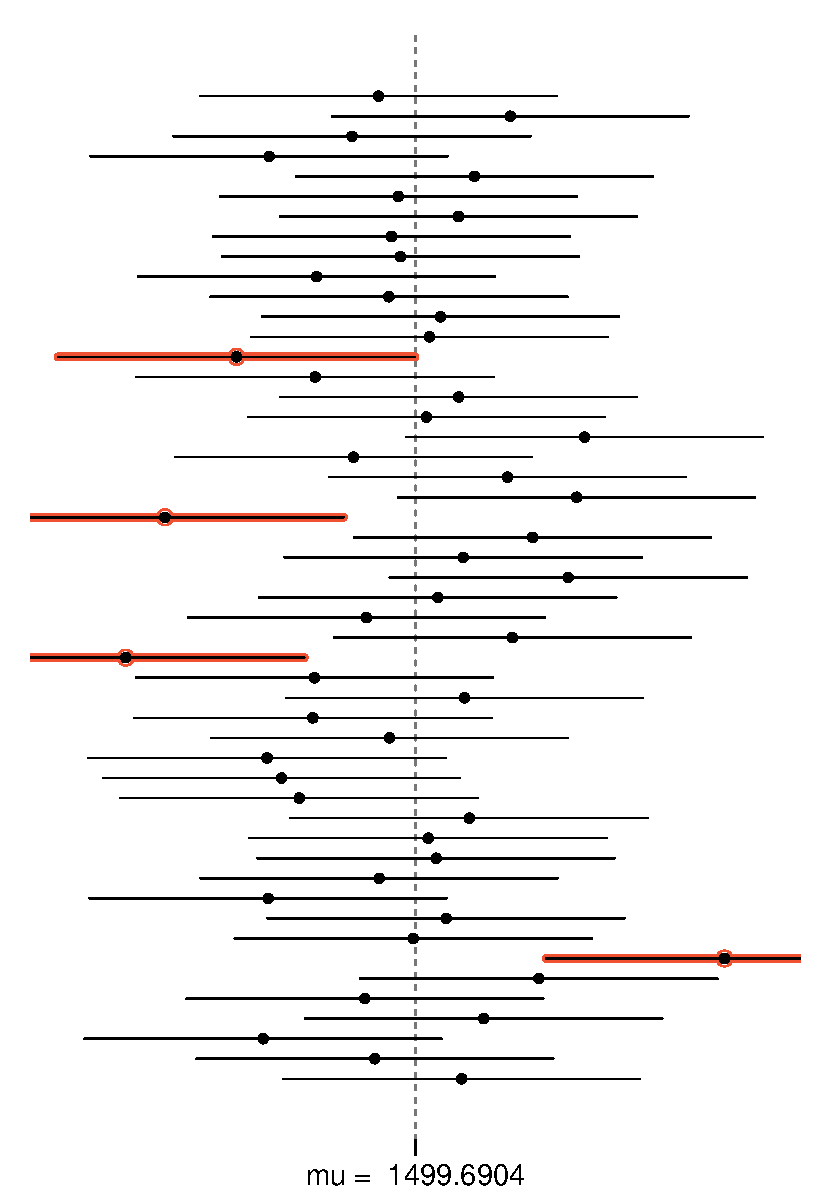
\includegraphics[width=0.4\textwidth]{fig/ex4.pdf}
\end{figure}
\emph{Explanation: 예제 3의 1개의 랜덤표본이 아닌 50번의 랜덤표본의 추출과 신뢰구간을 결과를 도식화한 결과이다. 주어진 plot\_ci 함수를 활용하여 (lower, upper) 신뢰구간과 모평균의 비교를 가시화 할 수 있다. 빨간색으로 칠해진 도형은 평균을 포함하지 않는 신뢰구간이다 (5\% 확률).}  \\

\section*{Example 5}
평균이 3이고 분산이 81인 $N(3,81)$에서 100개, 1,000개, 10,000개의 샘플들을 \texttt{x1}, \texttt{x2}, \texttt{x3}에 저장하여라. 각 \texttt{x1}, \texttt{x2}, \texttt{x3}의 평균과 분산을 구하여라. 어떤 경우가 원래의 평균과 분산에 더 가까운가? 샘플 수를 더 늘릴때는 어떻게 될지 간단히 서술하시오.
\begin{lstlisting}[style={r-style}]
set.seed(202011)
mu = 3; sigma = 9
x1 = rnorm(100, mu, sigma)
x2 = rnorm(1000, mu, sigma)
x3 = rnorm(10000, mu, sigma)
mean(x1); sd(x1)^2
mean(x2); sd(x2)^2
mean(x3); sd(x3)^2
\end{lstlisting}
\begin{lstlisting}[style={out-style}]
[1] 2.791411
[1] 90.76621

[1] 3.228978
[1] 75.43125

[1] 2.93461
[1] 81.00428
\end{lstlisting}
\emph{Explanation: 평균이 3이고 표준편차가 9인 정규분포에서 랜덤샘플을 갯수에 맞게 rnorm() 함수를 통해 추출하여 이를 x1, x2, x3에 저장하고 각각에 대한 평균과 표준편차를 계산하였다. 샘플의 갯수가 가장 큰 x3의 경우 모평균과 모분산과 가장 가까웠으며 샘플 수를 늘릴수록 더욱 가까워질 것으로 예상된다. } \\

\section*{Example 6}
추정치가 몇개의 신뢰구간에 포함되는지 알아보고자 한다. 평균이 3이고, 분산이 81인 $N(3,81)$에서 10개 샘플을 뽑고 $\alpha=0.05$일때의 신뢰구간을 구한다. 이 과정을 100번 수행하여 총 신뢰구간 100개를 구하여라. 이때 원래 평균값인 3이 포함되는 신뢰구간의 개수는 몇개인가? 
\begin{lstlisting}[style={r-style}]
set.seed(202011)
mu = 3; sigma = 9; n = 10; alpha = 0.05
count = 0
for (i in 1:100) {
  sample = rnorm(n, mu, sigma)
  hi = mean(sample) + qnorm(1-alpha/2)*(sigma/sqrt(n))
  lo = mean(sample) - qnorm(1-alpha/2)*(sigma/sqrt(n))
  if ((lo < mu) && (mu < hi)) count = count + 1
}
count
\end{lstlisting}
\begin{lstlisting}[style={out-style}]
[1] 96
\end{lstlisting}
\emph{Explanation: 주어진 정규분포를 따르는 랜덤 표본은 rnorm() 함수를 통해 sample에 저장한 후 각각의 모평균에 대한 95 \% 신뢰구간을 연산하여 모평균이 이 구간에 들어갈 경우를 if 문 처리를 통해 count를 하나씩 증가시켰다. 이 때 모평균 3이 표한되는 신뢰구간의 갯수는 100개 중 96개로 96 \%이다.} \\

\section*{Example 7}
어떤 물질 X는 흔하지만, 농도를 정확하게 검출하는 것이 힘들다. A는 21번의 실험을 통해서 X의 농도를 측정하였다. 측정된 농도는 다음과 같다.
\newline
\fbox{\begin{minipage}{\textwidth}
78.70, 83.43, 76.19, 77.70, 78.54, 81.66, 78.42,
81.54, 79.37, 78.24, 76.28, 79.41, 79.95, 80.44,
77.94, 78.18, 78.54, 78.39, 79.27, 80.07, 81.07
\end{minipage}}
\newline
이 자료를 본 B는 평균이 79라고 주장하였고, C는 평균은 79를 넘는다고 주장하였다.
\begin{equation*}
H_0: \mu=79 \quad H_1: \mu>79
\end{equation*}
이 가설에 대하여 검정통계량의 값을 구하고, p-value를 구하시오. (X의 모표준편차는 2로 가정한다.) 
\begin{lstlisting}[style={r-style}]
X.sample = c(78.70, 83.43, 76.19, 77.70, 78.54, 81.66, 78.42, 
             81.54, 79.37, 78.24, 76.28, 79.41, 79.95, 80.44, 
             77.94, 78.18, 78.54, 78.39, 79.27, 80.07, 81.07)
n = length(X.sample)
X.mu = 79; X.sigma = 2
z = (mean(X.sample) - X.mu) / (X.sigma/sqrt(n)); z
pvalue = pnorm(z, lower.tail=F); pvalue
\end{lstlisting}
\begin{lstlisting}[style={out-style}]
[1] 0.4724417
[1] 0.3183058
\end{lstlisting}
\emph{Explanation: 21번의 실험을 통해 측정한 물질 X의 검출 농도를 X.sample 벡터에 저장하였다. 모분산을 알고 있으므로 귀무가설 하의 검정 통계랑을 표준 정규분포 통계량 z로 설정할 수 있다. 우측 검정이므로 pnorm() 함수를 통해 lower.tail이 아닌 upper.tail의 누적확률분포값을 이용해 유의확률 0.3183을 구할 수 있다. 통상적으로 많이 쓰이는 유의수준 $\alpha = 0.05$에 비해 훨씬 큰 값이므로 대립가설을 채택하기 어렵다고 결론 지을 수 있다. } \\

\end{document}
